\section{Statistics}\label{sec:statistics}

Every science starts from a hypothesis to be tested. The task is to make a statement if the proposed hypothesis agrees or disagrees with observed data, to either accept or reject it against the null-hypothesis. The metric at hand to do so is the p-value that arises within hypothesis testing. 

For exactly this task high energy physicists have developed a framework based on likelihood statistics tailored for counting experiments. This section begins to lay out the fundamentals of the approach and then goes to the hands on implementation of its use. The following is based on \citep{cowan2011asymptotic,behnke2013data,pyhf_intro}.

\subsection{Building the likelihood}
As we are dealing with a counting experiment the tool at hand are histograms $\bm{n}=(n_1,...,n_N)$. It can be modeled with a set of parameters divided into so called parameters of interest, here only the signal strength $\mu$, and nuisance parameters $\bm{\Theta}$, that basically serve to give the model flexibility to fit the observations. The bin heights (counts) can then be expressed in terms of the amount of signal $s_i(\bm{\Theta})$ and background $b_i(\bm{\Theta})$ in them. The expectation value of the $n_i$ is then
\begin{equation} \label{eq:n_i}
    \langle n_i(\mu,\bm{\Theta})\rangle = \mu s_i(\bm{\Theta}) +b_i(\bm{\Theta}).
\end{equation}
The model can be further constrained with auxiliary histograms $\bm{a}=(a_1,...,a_M)$ with bin height
\begin{equation} \label{eq:a_i}
    \langle a_i(\bm{\Theta}) \rangle = u_i(\bm{\Theta}).
\end{equation}
As we are expecting the bin counts to occur with a constant mean rate and independent of time compared to the last event each follows a Poisson distribution
\begin{equation}\label{eq:poisson}
    \frac{r^k e^{-r}}{k!}.
\end{equation}
$r$ is the expected rate of occurrences, which translates as our prediction, whereas $k$ are the actual measured occurrences. From this a likelihood $L(\bm{x})$ can be built, which is just a probability under a given set of parameters $\bm{x}$. Accounting for all the bins by multiplying them together yields
\begin{equation}
    L(\mu,\bm{\Theta})=
    \prod_{j=1}^N \frac{(\mu s_j + b_j)^{n_j}}{n_j !} e^{-(\mu s_j + b_j)}
    \prod_{k=1}^M \frac{u_k^{a_k}}{a_k!} e^{-u_k}.
\end{equation}
To test for a hypothesized value of $\mu$, the best choice according to the Neyman-Pearson lemma, is the profile likelihood ratio that reduces the dependence to one parameter of interest $\mu$
\begin{equation}
\lambda(\mu)=
    \frac{L(\mu,\hat{\hat{\bm{\Theta}}})}
    {L(\hat{\mu},\hat{\bm{\Theta}})}
\end{equation}
The denominator is the unconditional maximum likelihood estimation so that $\hat{\mu}$ and $\hat{\bm{\Theta}}$ both are free to vary to maximize $L$. Whereas the numerator is the found maximum likelihood conditioned on some chosen $\mu$ and the set of found nuisance parameters $\hat{\hat{\bm{\Theta}}}$ that maximize the likelihood. This definition gives $0 \leq \lambda \leq 1$. For a $\lambda \sim 1$ the hypothesized value of $\mu$ shows good agreement to the Poissonian model.

\subsection{From test statistic to p-value}   
Transforming the profile likelihood into a test statistic $t_{\mu}$ is practical to calculate p-values
\begin{equation}
    t_{\mu}=-2\log \lambda(\mu).
\end{equation}
This translates as $t_{\mu} \rightarrow 0$ as good agreement, $t_{\mu} \rightarrow \infty$ as bad agreement to the model. A right-tail p-value can then be calculated from the probability density function of $t_\mu$: pdf$(t_\mu) = f(t_\mu \mid \mu)$
\begin{equation}\label{eq:p-value}
    p_\mu = \int_{t_{\mu ,obs}}^{\infty} 
    f(t_\mu \mid \mu) \mathrm{d}t_\mu
\end{equation}
$t_{\mu ,obs}$ is the test statistic $t_\mu$ evaluated at the observed data. This is like plugging into the Poisson distributions the same values for $r$ as for $k$ in eq. \ref{eq:poisson}. Just like a probability density function for a standard normal distribution, intuitively the pdf is just how probable is a particular value of the test statistic $t_\mu$ under a fixed value of the signal strength (how often it occurs compared to all other values $t_\mu$ can have). 

This particular form is handy because there exist approximations for $f(t_\mu \mid \mu)$ \citep{cowan2011asymptotic}. Wald \citep{wald1943tests} proved that in the large sample limit the test statistic follows a normalized sum of squared distances between the tested parameter of interest $\mu_i$ and its maximum likelihood estimate $\hat{\mu}_i$. The result was extended by Wilk \citep{wilks1938large} for any number of parameters of interest so the test statistic becomes
\begin{equation}
    t_\mu=\sum_i \frac{(\mu_i-\hat{\mu}_i^2)}{\sigma_i^2} + \mathcal{O}(1/\sqrt{N}).
\end{equation}
The $\hat{\mu}_i$ are in the large sample limit normally distributed with mean $\mu'$ (true values) and standard deviation $\sigma_i$. This basically the definition of a non-central chi-squared distribution with degrees of freedom equal to the parameters of interest (see section 3.1 in \citep{cowan2011asymptotic}). For one parameter of interest the distribution reads
\begin{equation}\label{eq:chi-square}
    f(t_\mu \mid \Lambda(\mu))=\frac{1}{2\sqrt{t_\mu}}\frac{1}{\sqrt{2\pi}}
    \left[
\exp\left(-\frac{1}{2}\left(\sqrt{t_\mu}+\sqrt{\Lambda}\right)\right)
+
\exp\left(-\frac{1}{2}\left(\sqrt{t_\mu}-\sqrt{\Lambda}\right)\right)
\right],
\end{equation}
with non-centrality parameter 
\begin{equation}
    \Lambda=\frac{(\mu-\mu')^2}{\sigma^2}.
\end{equation}
Figure \ref{fig:test_stat_example} illustrates the different steps. Being able to calculate p-values allows now to state how likely it is that the proposed hypothesis is reflected by the observed data. Put differently, if the experiment would be repeated the p-value represents the probability of obtaining a result that favors the alternative hypothesis over the null hypothesis. In the scientific community a widely accepted threshold for this is a p-value of 0.05. Though particle physicists only claim discovery of a new phenomenon for $p<$\SI{2.87e-7}{} (5 standard deviations of the standard normal distribution).

One caveat here is that this particular form of $t_\mu$ assumes $\mu$ can also be negative, which can be non-physical if one looks for a new process. Test statistics considering the different cases are covered in \citep{cowan2011asymptotic}. 
\begin{figure}
    \centering
    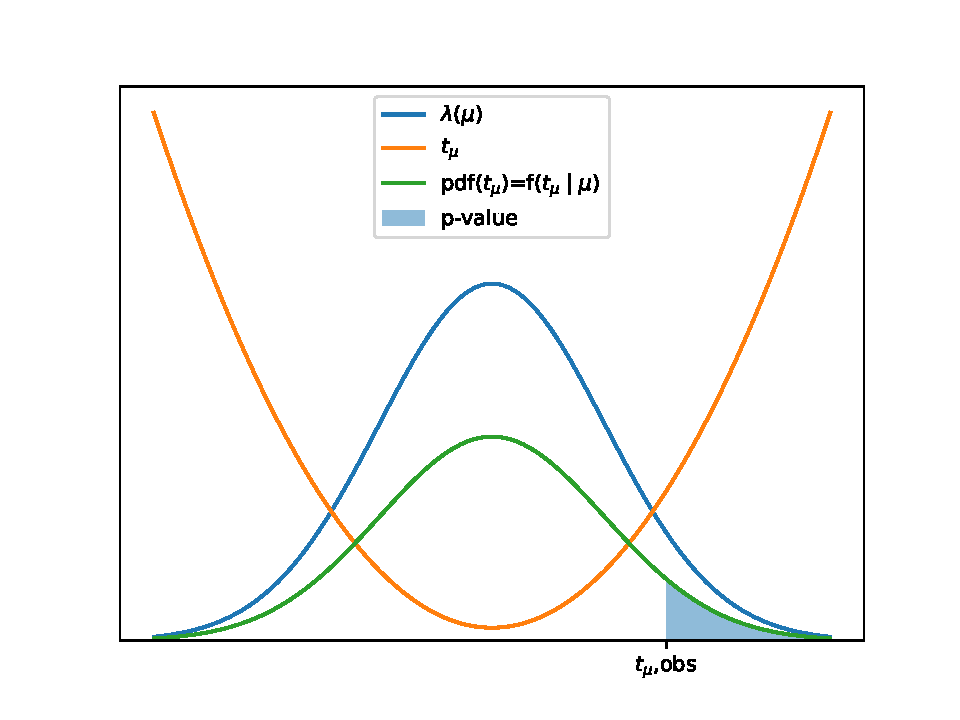
\includegraphics[width=0.8\textwidth]{test_stat_example.pdf}
        \caption[]{A sketch to follow the steps to calculate p-values. (\textbf{left}) The profile likelihood (\hexbox{1f77b4}) has essentially some hill-like form with a maximum at ${\lambda(\hat{\mu},\hat{\bm{\Theta}})}$, $t_\mu$ (\hexbox{ff7f0e}) is $-2\mathrm{ln}(\lambda)$. (\textbf{right}) For one parameter of interest in the large sample limit $f(t_\mu \mid \mu)$ follows a non-central chi-squared distribution with one degree of freedom, equation \ref{eq:chi-square}. The blue shaded area under the pdf is a right hand sided p-value.}
    \label{fig:test_stat_example}    
\end{figure}

\subsection{The CL$_s$ value}\label{sec:cls}

Particle physicists are usually interested in two things when making statistical tests for discovery of new phenomena: how well is the modeling of backgrounds (things we know) and if there is evidence in the observations for a new phenomenon. This means one needs to test two hypotheses: a background only ($b$) and a signal plus background ($s+b$) hypothesis. Each will result in a p-value on their own. For example $p_{b}=0$ would mean that the backgrounds are perfectly reflected by the observations and a $p_{s+b} < 0.05$ could be a sign of e.g. new physics. To combine these two metrics into a single score, particle physicists came up with the pseudo Confidence Level/p-value called CL$_s$ incorporating also the goodness of the modeling of the backgrounds 
\begin{equation}
    \mathrm{CL}_s=\frac{p_{s+b}}{1-p_{b}}=
    \frac
    {\int_{t_{\mu ,obs}}^{\infty} 
    f(t_\mu \mid \mu) \mathrm{d}t_\mu}
    {1-\int_{t_{\mu ,obs}}^{\infty} 
    f(t_\mu \mid \mu) \mathrm{d}t_\mu}.
\end{equation}
Intuitively the numerator is again just the value for the alternative hypothesis whereas the denominator penalizes CL$_s$ if the modeling of the backgrounds is not reflected in the observations. This can also be understood visually from the first figure of the heavily cited CL$_s$ paper \citep{read2002presentation} (see description of fig. \ref{fig:cls}).
\begin{figure}
    \centering
    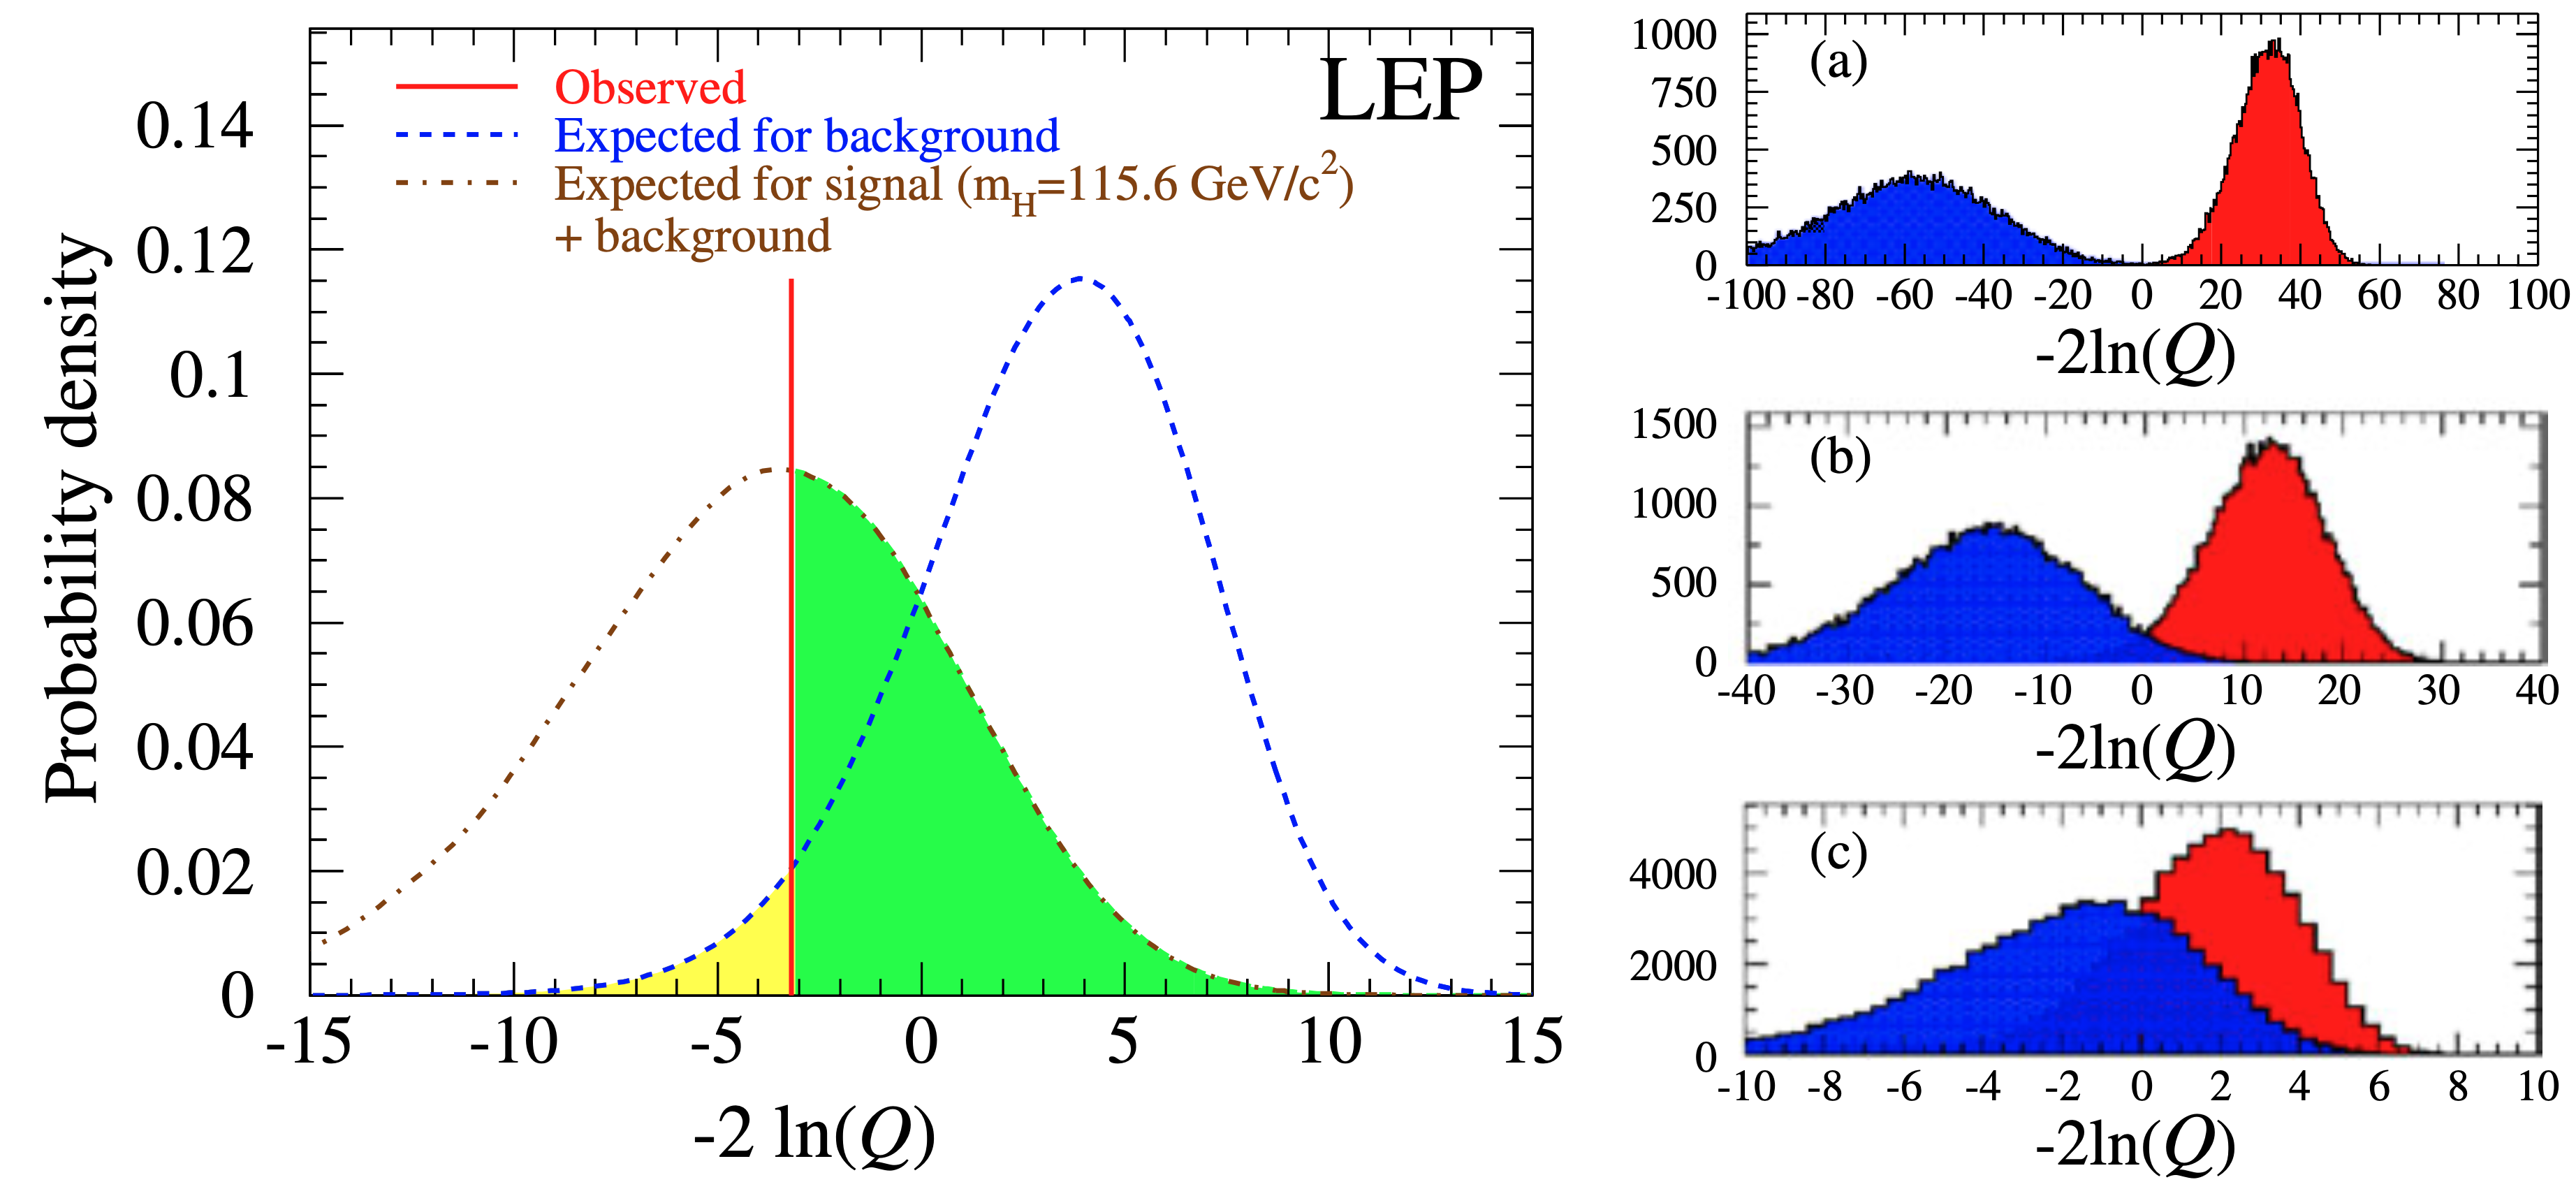
\includegraphics[width=1\textwidth]{cls.png}
        \caption[]{Probability density functions of test statistics from a Higgs search at LEP illustrating the calculation of p-values ($\lambda$ becomes $Q$). (\textbf{left}) The pdf's of the test statistic $f(t_\mu \mid \mu)$ of the signal + background ({\color[HTML]{804000}{$\diagup$}}) and background ({\color[HTML]{2100FF}{$\diagup$}}) only hypotheses. The p-value is calculated by integration from $t_{\mu,obs}$ (the red observed line ({\color[HTML]{FF0000}{$\diagup$}})) to infinity (see eq. \ref{eq:p-value}). The green shaded area (\hexbox{00FF00}) corresponds to $p_{s+b}$ whereas the yellow area (\hexbox{FDFF02}) corresponds to $1-p_b$ since the integral over one whole pdf is 1. (\textbf{right}) Degradation of search sensitivity from (a) to (c). Note that the colors of the pdf's change here to signal + background (\hexbox{2100FF}) and background only (\hexbox{FF0000}). For example putting the observation on the x-axis at 0 in these plots, one would get for plot (a) $p_{b}\approx 1$ and $p_{s+b}\approx 0$ resulting in a CL$_s\approx 0$, whereas with increasing overlap the CL$_s$ value increases and the sensitivity decreases.
        From \citep{read2002presentation}.}
    \label{fig:cls}    
\end{figure}



\subsection{Histfactory in pyhf}



Detector-simulation related uncertainty
– Calibrations (electron, jet energy scale)
– Efficiencies (particle ID, reconstruction)
– Resolutions (jet energy, muon momentum)!
!
• Theoretical uncertainties
– Factorization/Normalization scale of MC generators
– Choice of MC generator (ME and/or PS, e.g. Herwig vs Pythia)
• Monte Carlo Statistical uncertainties
– Statistical uncertainty of simulated samples

